\section{Editor}
\label{sec:editor}

\begin{figure}[htb]
    \centering
    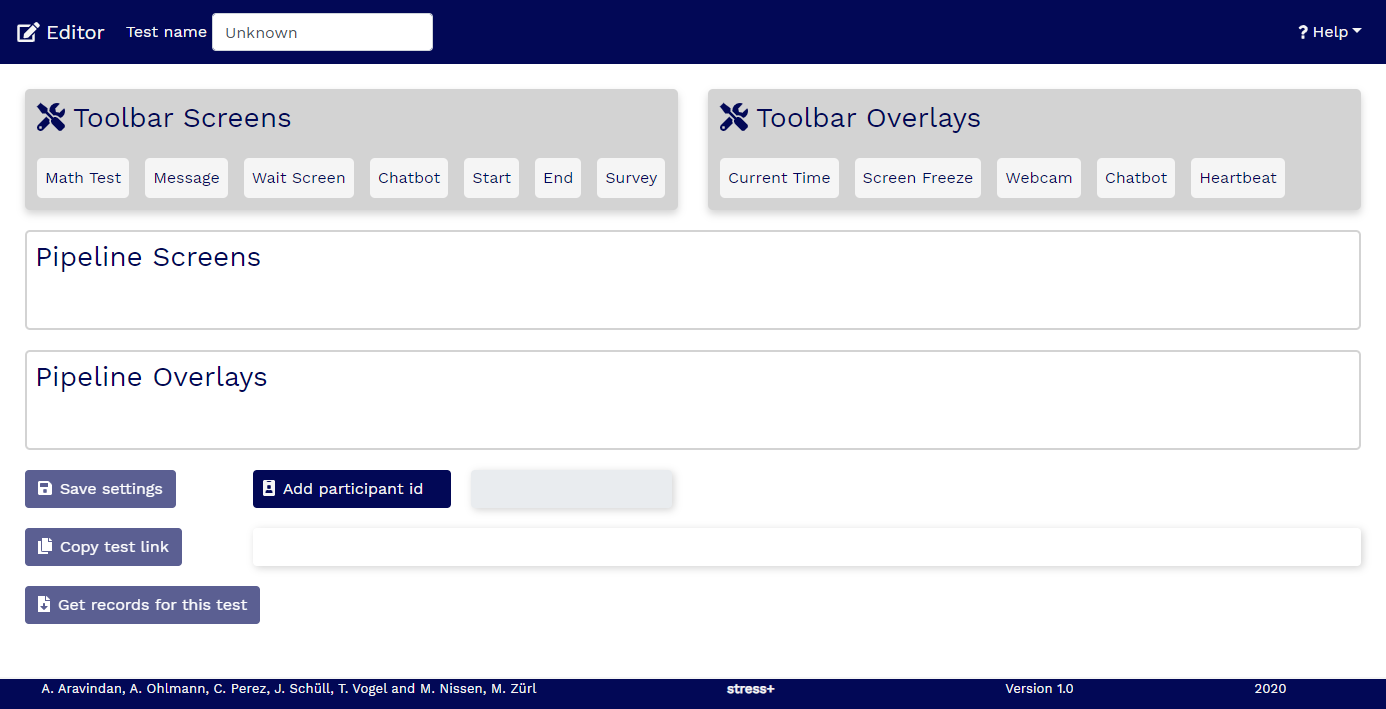
\includegraphics[width=\textwidth]{figures/screenshot-editor.png}
    \caption{Screenshot of the editor after creating a new stress test}
    \label{fig:screenshot-editor}
\end{figure}

Figure \ref{fig:screenshot-editor} shows a screenshot of the editor after creating a new stress test.

The stress test can be created and edited in the editor with dragging and dropping items from a toolbar to the pipeline.
The editor has one toolbar for the screens and one for the overlays. 
There are also two separate pipelines for the screens and the overlays. 
Within each item inside a pipeline the user can adjust the settings of the current item. 
Stress test do have a name that can be changed inside the editor.
Each stress test has a unique ID that is generated when it is saved for the first time.
With this ID a link is generated that can be send to patients so they can execute the stress test.
The UI also allows the user to download all statistics for the current stress test.
